\documentclass[a0,portrait]{a0poster}
%\documentclass{sciposter}
\usepackage[spanish]{babel}%Formata as entradas para PT-BR
%\usepackage[utf8]{inputenc}
%\usepackage{verbatim}
\usepackage[document]{ragged2e}
\usepackage{multicol} % This is so we can have multiple columns of text side-by-side
\columnsep=100pt % This is the amount of white space between the columns in the poster
\columnseprule=3pt % This is the thickness of the black line between the columns in the poster

\usepackage[svgnames]{xcolor} % Specify colors by their 'svgnames', for a full list of all colors available see here: http://www.latextemplates.com/svgnames-colors

\usepackage{times} % Use the times font
%\usepackage{palatino} % Uncomment to use the Palatino font
%\usepackage{varioref}
%\usepackage{hyperref}
%\usepackage{epsfig}
\usepackage{graphicx} % Required for including images
%\graphicspath{{figures/}} % Location of the graphics files
\usepackage{subfigure}
\usepackage{float}
\usepackage{booktabs} % Top and bottom rules for table
\usepackage[font=small,labelfont=bf]{caption} % Required for specifying captions to tables and figures
\usepackage{amsfonts, amsmath, amsthm, amssymb} % For math fonts, symbols and environments
\usepackage{mathrsfs}
\usepackage{wrapfig} % Allows wrapping text around tables and figures
\usepackage{setspace}
\usepackage{tabularx}
\usepackage{lipsum}
\usepackage{thmtools}%algoritmo
\setlength\parindent{0pt}
\usepackage[ruled,norelsize]{algorithm2e}
\makeatletter
\newcommand{\removelatexerror}{\let\@latex@error\@gobble}
\makeatother
\usepackage[framed,autolinebreaks,useliterate]{mcode}
\usepackage{listings}% http://ctan.org/pkg/listings
\renewcommand{\lstlistingname}{Código}% Listing -> Algorithm
\usepackage{algorithmic}

%

\begin{document}
\onehalfspacing
%----------------------------------------------------------------------------------------
%	POSTER HEADER 
%----------------------------------------------------------------------------------------

% The header is divided into two boxes:
% The first is 75% wide and houses the title, subtitle, names, university/organization and contact information
% The second is 25% wide and houses a logo for your university/organization or a photo of you
% The widths of these boxes can be easily edited to accommodate your content as you see fit

\begin{center}
	%\hspace*{-1.6cm}

\includegraphics[width=0.9\textwidth]{imagenes/Encabezado_Poster_ALTENCOA11_2026MathSiCA.png}
\end{center}
\quad\\
\begin{minipage}[b]{1.0\linewidth} %default 0.75
\begin{center}
{
\Huge \textbf{Fractales y autómatas celulares: Exploración computacional}
}\\[0.2cm]

\Large \textbf{Juan David Tarapuez} - \Large \texttt{jtarapuez24b\@udenar.edu.co}\\

\Large \textbf{Andres Camilo Enriquez} - \Large \texttt{acenriquez24b\@udenar.edu.co}\\

\Large \textbf{Alvaro Yussed Enriquez} - \Large \texttt{ayenriquez24b\@udenar.edu.co}\\

\Large \textbf{Asesora: } Catalina M. Rúa-Alvarez (UDENAR)\\

\huge Física, Universidad de Nari\~no, Pasto\\
\end{center}
\end{minipage}
%
\vspace{0.12cm} % A bit of extra whitespace between the header and poster content
%----------------------------------------------------------------------------------------
\begin{multicols}{3} % This is how many columns your poster will be broken into, a portrait poster is generally split into 2 columns
\justify % Justify all text
\vspace{-1.2cm}
\section{Introducción}

La geometría fractal permite el estudio de estructuras complejas y 
autosimilares mediante procesos iterativos. Esta investigación aborda 
la transición de estos sistemas desde el plano bidimensional hacia el 
espacio tridimensional mediante los siguientes enfoques:

 \begin{itemize}
    \item \textbf{Triángulo de Sierpinski}: Construcción bidimensional iterativa 
    generada al reducir un triángulo equilátero a su cuarta parte y 
    posicionar tres figuras a escala, formando un patrón continuo de 
    autosimilitud.

    \item \textbf{Tetraedro de Sierpinski y dimensión fractal}: Generalización 
    tridimensional mediante un algoritmo que ensambla cuatro copias de un tetraedro 
    regular con sus aristas reducidas a la mitad. Esta extensión resalta el papel de 
    la dimensión fractal para describir la complejidad espacial y facilita el 
    análisis de la evolución del área hacia el volumen.

    \item \textbf{Construcción Computacional:} Diseño de un pseudocódigo basado 
    en llamadas recursivas que utiliza como parámetros la longitud de la arista, 
    el punto inicial y el número de iteraciones para visualizar matemáticamente 
    la estructura generada.
 \end{itemize}
\vspace{0.2cm}


 pus\section{Dimensión de Hausdorff y Autosimilitud}

El Triángulo de Sierpinski (Figura \ref{sierspinsky}) es un objeto \textbf{autosimilar}: al acercarnos a cualquier parte de su interior, reencontramos la misma estructura original. Para caracterizar geométricamente este tipo de objetos, utilizamos la \textbf{Dimensión de Hausdorff}, que responde a la pregunta: \textit{¿Cuánto espacio llena realmente la figura?}

Es importante matizar que la autosimilitud no implica directamente que un objeto sea un fractal, así como no todos los fractales son estrictamente autosimilares.

\subsection{Intuición geométrica del espacio}

Consideremos objetos clásicos de longitud 1 y dividámoslos en fragmentos de tamaño $\frac{1}{n}$:
\begin{itemize}
    \item \textbf{Segmento (1D):} Para rellenarlo necesitamos $N = n^1$ copias.
    \item \textbf{Cuadrado (2D):} Para rellenarlo necesitamos $N = n^2$ copias.
    \item \textbf{Cuadrado (3D):} Para rellenarlo necesitamos $N = n^3$ copias.
\end{itemize}

En general, el número de fragmentos $N(n)$ requeridos se relaciona con el factor de división $n$ mediante un exponente $d$ (la dimensión hipotética):
\begin{equation}
    N(n) = n^d
\end{equation}

\subsection{Cálculo de la dimensión hipotética}

Aplicando logaritmos y despejando $d$, obtenemos una dimensión que no necesita ser un número entero:
\begin{equation}
    d = \frac{\log(N(n))}{\log(n)}
    \label{eq:dim_similitud}
\end{equation}

\subsection{Generalización en el límite}

Para medir un área compleja $A \subset \mathbb{R}^2$, contemplando solapamientos y recubrimientos de regiones externas a $A$, la teoría de Hausdorff se basa en recubrir $A$ con sucesiones finitas numerables de conjuntos de diámetros infinitesimales ($x_i \to 0$) \cite{Gustavo}. Al tomar el límite, la dimensión fractal se define formalmente como:
\begin{equation}
    d = \lim_{n \to \infty} \frac{\log(N(n))}{\log(n)}
    \label{eq:dim_hausdorff}
\end{equation}
Este límite nos permite calcular la dimensión exacta de fractales geométricos mediante su escala de recubrimiento.



\vspace{0.2cm}

\section{Triángulo de Sierpinski}

El proceso para construir el triángulo de Sierpinski consta de reducir el tamaño de un tríangulo equilátero a su cuarta parte de forma que su lado sea la mitad de su lado original, se posicionan tres figuras iguales a esta de manera que formen otro triángulo de lado igual al original. Se repite el mismo proceso para los tres triánguos formados y se vuelve a hacer para todos los nuevos triángulos generados en cada iteración. \cite{Gustavo}

\begin{figure}[H]
    \centering
    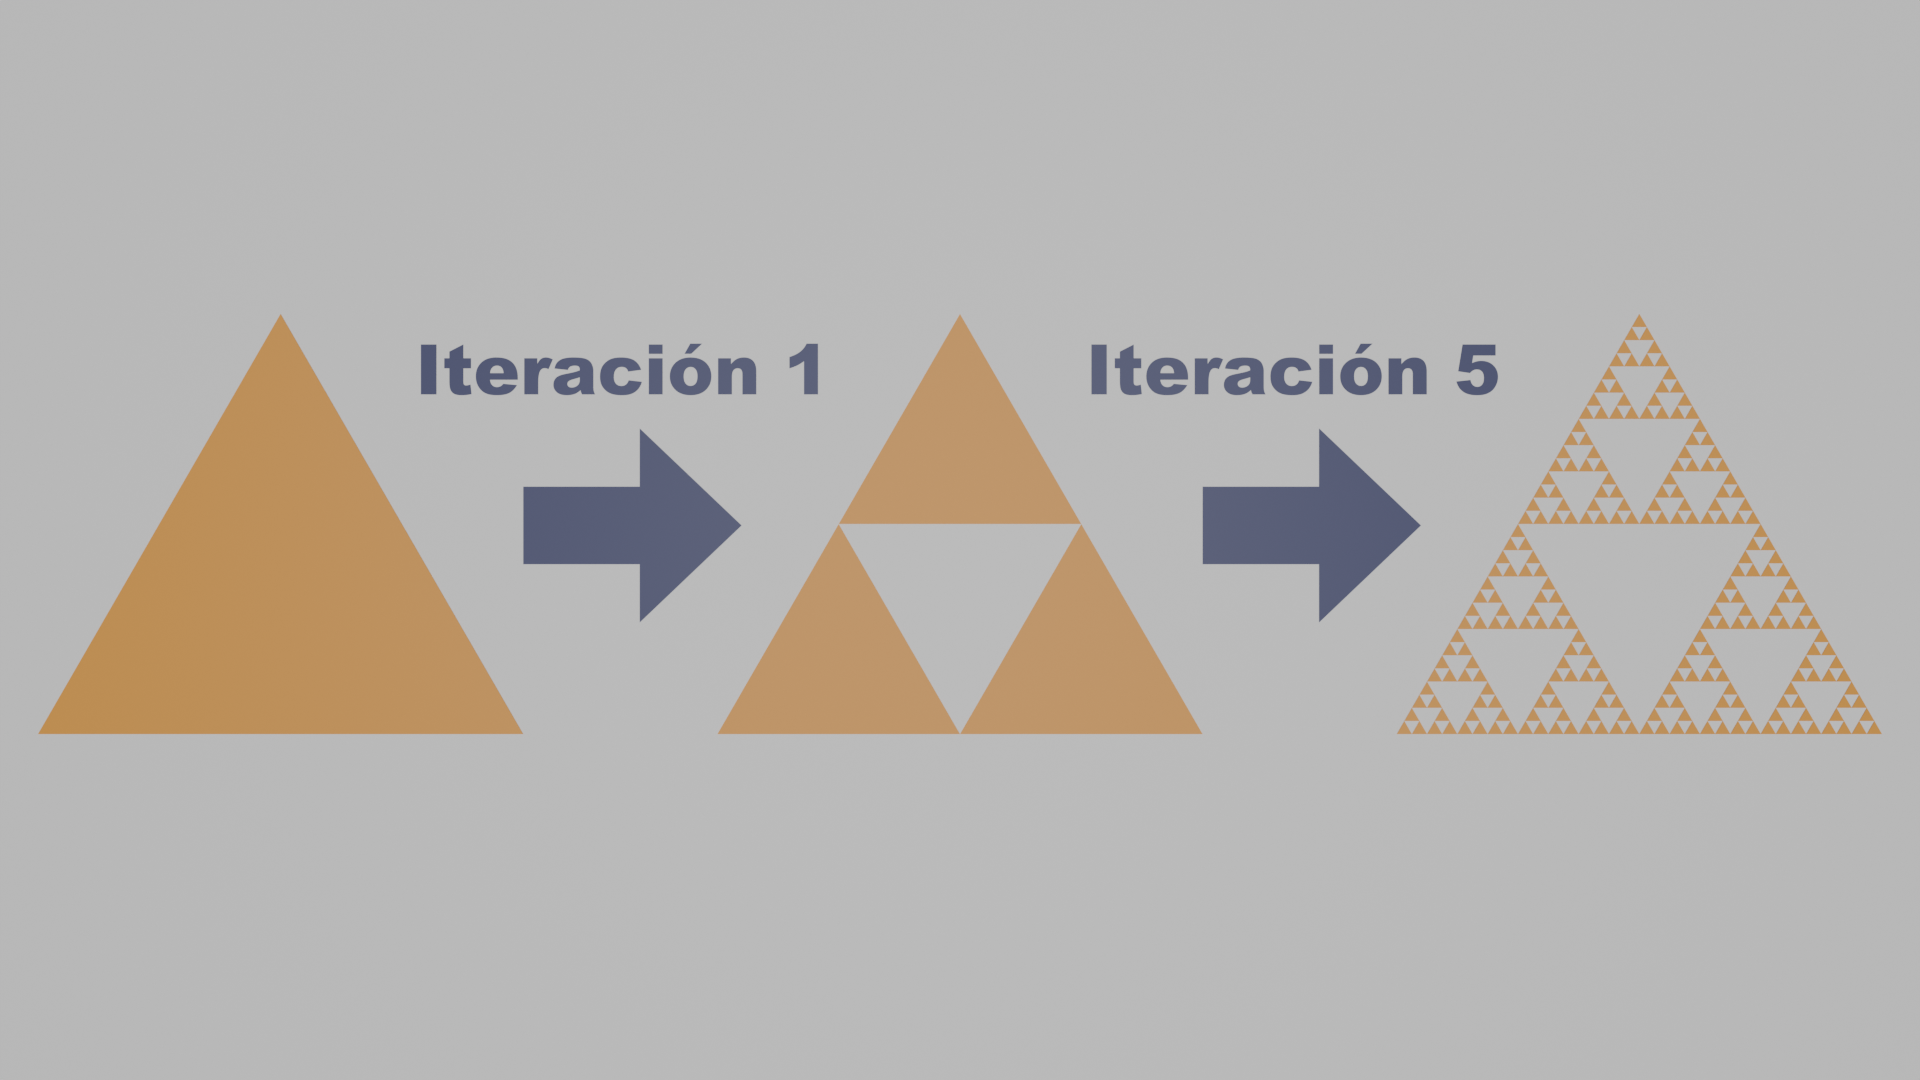
\includegraphics[width=0.5\linewidth]{Figuras/Triangulo.png}
    \caption{Construcción del triángulo de Sierpiński mediante iteraciones sucesivas. Se muestra el triángulo inicial, la primera iteración y la quinta iteración del proceso.}
    \label{fig:triangulo-sierpinski}
\end{figure}
\vspace{0.2cm}

\input{capitulos/propiedades.tex}
\vspace{0.2cm}

\section{Tetraedro}

Para formar el tetraedro se sigue un algoritmo análogo al proceso que se usa para formar el triángulo. Se unen los puntos medios de las aristas de un tetraedro regular formando 8 tetraedros nuevos, luego se extraen 4 de ellos dejando los posicionados en las esquinas de la figura original. Se repite este mismo proceso para los nuevos tetraedros generados en cada iteración.

Para formar el tetraedro se sigue un algoritmo análogo al proceso que se usa para formar el triángulo. Se reduce un tetraedro regular a su octava parte de forma que su arista sea la mitad de su arista original, se posicionan cuatro figuras iguales a esta de manera que formen otro tetraedro de arista igual a la original. Se aplica lo mismo a cada nuevo tetraedro y se vuelve a repetir para cada nuevo tetraedro formado en cada iteración.
\vspace{0.2cm}

\section{Pseudocodigo}

Para generar la pirámide se usó el siguiente algoritmo, basado en el algoritmo para generar el triángulo:

\begin{algorithmic}
	\REQUIRE Longitud de arista ($L$), coordenadas punto inicial ($P_0$), número de iteraciones ($n$)
	\ENSURE Pirámide de Sierpinski
	\STATE $P_1 \gets [P_0[0]+L,   P_0[1],              P_0[2]]$
	\STATE $P_2 \gets [P_0[0]+L/2, P_0[1]+L*3**(1/2)/2, P_0[2]]$
	\STATE $P_3 \gets [P_0[0]+L/2, P_0[1]+L*3**(1/2)/6, P_0[2]+L*6**(1/2)/3]$
	\IF{$n == 0$}
		\STATE $[P_0, P_1, P_2, P_3] \gets PiramideRegular$
	\ELSE
		\STATE PiramideSierpinski($L/2, P_0, n-1$)
		\STATE PiramideSierpinski($L/2, [P_0[0]+L/2, P_0[1],              P_0[2]], n-1$)
		\STATE PiramideSierpinski($L/2, [P_0[0]+L/4, P_0[1]+L*3**(1/2)/4, P_0[2]], n-1$)
		\STATE PiramideSierpinski($L/2, [P_0[0]+L/4, P_0[1]+L/48**(1/2),  P_0[2]+L*6**(1/2)/6], n-1$)
	\ENDIF
\end{algorithmic}
\vspace{0.2cm}



\begin{multicols}{2}


\vspace{0.5cm}
  
\end{multicols}

\nocite{*} 
\end{multicols}

\textbf{Referencias: }

\vspace{-0.3cm}
[1] Diaz, A. C., Rúa-Alvarez, C. M. \& Rodriguez, P. M. \textit{On a
general model of rumor transmission}. Proceeding Series of the Brazilian
Society of\\\vspace{-0.2cm}Computational and Applied Mathematics, 8(1):1–2 (2021). 

\vspace{-0.1cm}[2] Guerrero, D. J., Rúa-Alvarez, C. M. \& Castillo, J. H.  
\textit{Fractales, Matemáticas y Algoritmos}.  Informe final, Universidad de Nariño (2023). 

\vspace{-0.1cm}[3] Sabogal, S. \& Arenas, G. \textit{Una introducción a la geometría fractal}. Universidad Industrial de Santander, Ediciones UIS (2011).

\vspace{-0.1cm}[4] Terán, J. A.  \textit{Generalización del método de Newton y sus aplicaciones}.  Tesis de Pregrado, Universidad de Nariño, Pasto (2018).

\vspace{-0.1cm}[5] Terán, J. A. \& Rúa-Alvarez, C. M. \textit{El método de Newton para raíces complejas: Fractales en el problema de Cayley}.  Revista EIA, 15(29):97–108 (2018).

\vspace{-0.1cm}[6] Wolfram, S. \textit{A New Kind of Science}.  Wolfram Media, Champaign, Illinois (2002).
\end{document}